\documentclass[12pt]{article}
\usepackage[letterpaper, margin=1in]{geometry} % [letterpaper, margin=1.25in]
\usepackage[english]{babel}
\usepackage[utf8]{inputenc}
\usepackage{todonotes}
\usepackage{fancyhdr}
\usepackage{booktabs}
\usepackage{graphicx}
\usepackage{lastpage}


\usepackage{hyperref}

\pagestyle{fancy}
\fancyhf{}
\rhead{Paras Jain // pjain67}
\lhead{CS4641 Project 2: Randomized Optimization}
\cfoot{\thepage}

\title{CS4641: Randomized Optimization}
\author{Paras Jain}
\date{March 2016}

\begin{document}

\maketitle




\section{Phase 1: Training a neural network}
\subsection{Dataset for Neural Network training}
From Project 1, I continue to use the political party voting dataset. As a recap from Project 1, the voting dataset classifies 1984 congresspersons as Republican or Democrats based on their votes. The data was stored in ARFF format, which ABIGAIL\footnote{\url{https://github.com/pushkar/ABAGAIL}} can import. The data contains 16 discrete binary features and 1 discrete binary label class (democrat/republican).

\subsection{Neural network training optimization problem}
A neural network is trained using the various optimization algorithms rather than using backpropagation. In order to actually create an optimization problem, the output layer of a neural network is scored with a cost function (Sum of Squares). This allows optimization algorithms to optimize the domain of the problem (weights of the neural network) in order to minimize the cost, thereby minimizing training error. The optimal hyperparameters were kept constant from Project 1.

\subsubsection{Continuous domains}
Many of these optimization problems work well over discrete domains as compared to the continuous domain of neural network weight paramater optimization. Several methods can be use to optimize problems over continuous domains including discretizing them. However, each of these methods have their own tradeoffs.
Generally, it will take longer to converge on an optimal solution over a continuous domain as compared to a discrete domain. Comparing Phase 1 and Phase 2, it's clear that these algorithms stuggle more over continuous domains as compared to discrete domains. This makes sense as there are potentially an infinite number of possible values for each parameter compared to finite number of discrete parameters.

\subsection{Optimization algorithms}
Many of these optimization algorithms are already implemented in ABIGAIL, which was used by the experiment runners. Performance is defined by $\frac{TP+TN}{TP+TN+FP+FN}$ from the confusion matrix. More simply, this is $\frac{correct\ classifications}{incorrect\ classifications}$

\subsubsection{Randomized hill climbing}
Randomized Hill Climbing searches for maxima by climbing hills of the cost function, or going to the maximal neighbor at each time step. In order to avoid getting stuck in local maxima, it utilizes random restarts in order to increase the probability that it reaches a global maximum. RHC\footnote{Randomized Hill Climbing} is not guaranteed to find the global maximum and can perform poorly depending on the cost function.


\subsubsection{Simulated annealing}
Simulated Annealing mathematically specifies the randomized behavior of escaping local maxima by modeling the process by which metals “anneal”. Temperature decreases over time reducing the probability that SA\footnote{Simulated Annealing} jumps to a sub-optimal point. SA can perform either well or poorly depending on the choice of temperature decay and tuning of other parameters.


\subsubsection{Genetic algorithms}
Genetic algorithms combine instances in order to maximize some kind of objective fitness function. GA\footnote{Genetic Algorithms} attempts to optimize the fitness function through crossover of models, which models natural selection. GA has several drawbacks in this optimization problem – the first is that optimizing a neural network is a continuous problem where weights are continuous variables. GA performs best on discrete optimization spaces. Moreover, sampling strategy and amount is very important, as it is important to capture a representative sample across the optimization space.  If a combination of the samples in the initial space cannot produce the desired maximum, then GA may perform sub-optimally.



\subsection{Results}

\subsubsection{Average performance}
\begin{figure}[h!]
    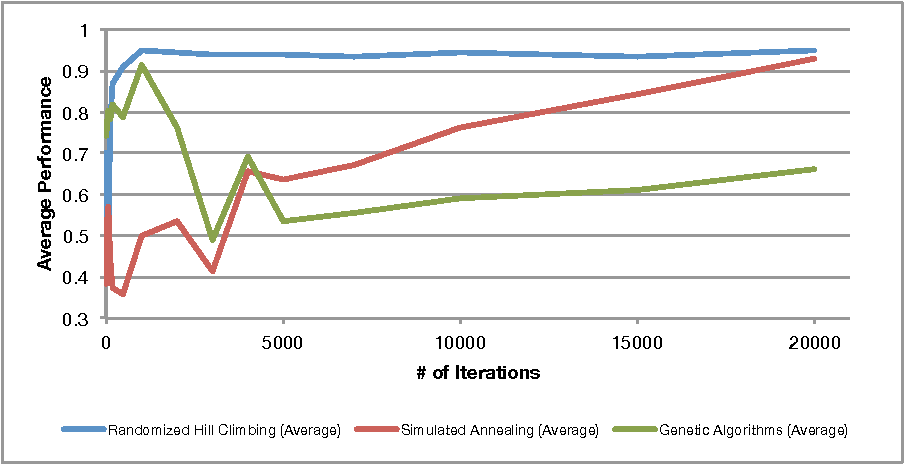
\includegraphics[width=\textwidth]{pics/AP}
    \caption{4 trial average test performance of various neural network optimization algorithms\footnote{This shows intermediate performance rather than max performance in order to show the evolution of each algorithm's behavior over time}}
    \label{fig:ap}
\end{figure}

In Figure \ref{fig:ap}, it is interesting to see how the different algorithms perform. RHC performs quite well and rapidly converges on an answer. Continued iterations fail to improve performance significantly. SA appears to vary considerably in the first 5000 iterations but appears to monotonically converge thereafter where it likely converged on a path near the global maxima. This result aligns with the functioning of the algorithm whereby it reduces the “temperature” as iterations increase.\footnote{Given an increased number of iterations, SA actually slightly exceeds the performance of RHC. This is not included in the chart as it disturbs the axis scale}  GA has a surprising result where it appears to not converge readily on the answer but instead only finds incremental performance improvement past the 5000th iteration. This behavior will be investigated further by varying parameters in a following experiment to study the effect of the population size on performance.

RHC performance was surprising as it performed well by converging quickly to an optimal solution. This may be due to the limited number of parameters in this model. This meant that randomly sampling throughout the optimization space was somewhat effective at converging on the global optimum quickly. As the cost function also has many small local maxima, RHC was effectively randomly sampling and testing points around the cost function. This result was surprising but makes sense perhaps given that RHC would be able to rapidly climb to the top of a peak after randomly happening on a path to the global maxima. I don't expect this performance to generalize as well to more difficult problems such as those seen in Phase 2.

SA performed best in the end\footnote{at 50,000 iterations, not shown on Figure \ref{fig:ap}} but converged much more slowly than RHC. Compare RHC's behviour of randomly sampling around the sample space to Simulated Annealing where it appears to struggle for a while to find a path to the global optimum but steadily converges on a solution after temperature decreased sufficiently. This can be controlled by adjusting the initial temperature and temperature cooling rate.

GA had trouble with this problem and it is not surprising given that there is no single primary dimension of the data so it's not necessarily the case that mixing weights will produce a more optimal set of weights. In the voting dataset, the features that give signal on political party are generally correlated. It's clear that GA struggles to converge. Perhaps a more intelligent crossover function could be used based on the domain knowledge of how neural network weights operate in order to get a more effective result. However, stock GA performs poorly. It trains for a large amount of time without significant performance improvements on the training dataset.

One interesting aspect of the data is the structure of features. As there are a fair number of features where some provide a large amount of information gain (bills where politicians vote along party lines) as compared to relatively low value features. Given some “levers” that do little to influence the result (low information gain attributes), various algorithms have different responses. This is one reason that genetic algorithms may perform poorly as some of the “levers” in the model do not represent a separate dimension of the resulting data. This hurts the performance of GA as the initial population may represent the space of models poorly.

Overfitting is interesting to examine. It appears that RHC did not overfit to the train dataset as test performance does not decrease over time. Given how clean the dataset was (as explored in Project 1), this does not surprise me as the test dataset should be very similar to the train dataset in structure. Also given how Project 1 uncovered that politicians tend to vote along party lines, there is not too much noise to overfit to. SA also shows no signs of overfitting but it may be that not enough iterations were run. Genetic algorithms appear to have begun to overfit very quickly - GA showed remarkable performance initially. I suspect this is because large of a initial population was chosen which meant that GA was effectively just randomly sampling across the cost function like RHC. Crossover reduced performance as the models absorbed too many details and subtleties of the training dataset. This is very interesting as backpropogation did not result in 

I suspect that there are a fair number of local optima, which would explain why GA and SA perform poorly. Factors that would contribute to this are the large number of features and the fact that some attributes roughly (but not exactly) correlate with each other.


\subsubsection{Optimizing temperature cooling rate}

\begin{figure}[h!]
    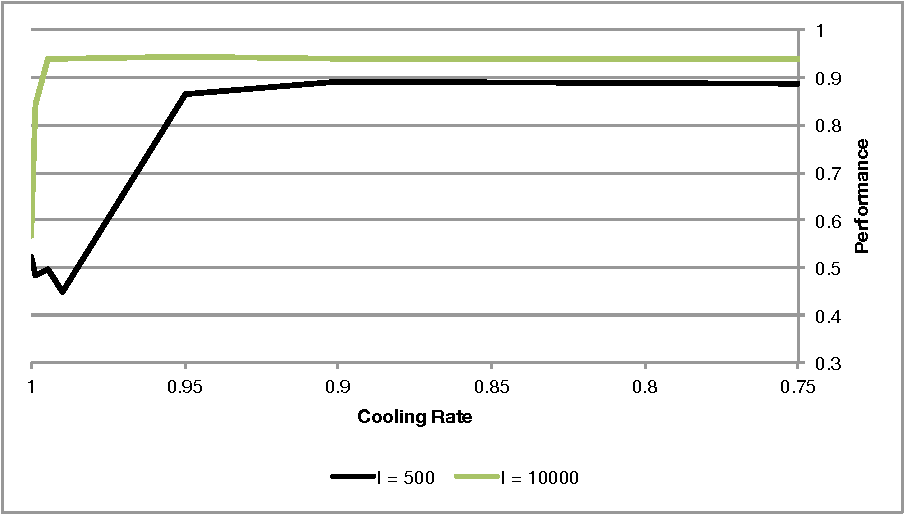
\includegraphics[width=\textwidth]{pics/coolingrate}
    \caption{Simulated Annealing Average Performance as a function of Cooling Rate}
    \label{fig:coolingrate}
\end{figure}

An experiment was conducted to determine the optimal cooling rate for Simulated Annealing. Through experimentation, I observed performance varied depending on the scale of cooling rate versus initial temperature (as compared to the raw values of each).

Iterations were fixed at 500 and 10000 in order to capture a snapshot-in-time picture of various values for the cooling rate. 15 trials were conducted and averaged to smooth out the resulting performance chart. Initial temperature is set to 10.

The results with this experiment, displayed in Figure \ref{fig:coolingrate}, are quite interesting – it appears that SA performs poorly with cooling rates very close to 1. This makes intuitive sense as this would make temperature decay slowly, which could cause SA to explore more perhaps sub-optimal areas. Interestingly, performance did not drop for lower cooling rates (closer to 0). These lower cooling rates should cause SA to converge faster. This implies that for cooling rate, there is a “good-enough” range of values for which it will perform. For values very close to 1, a large number of iterations are required in order to converge.

RHC seems to work well for the given optimization problem and a value of $0.95$ for the cooling value seems to be optimal as it has more room to grow but still converges to an optimal solution relatively quickly. As the number of iterations, almost all values for the cooling rate except for those very close to 1 converged.


\subsubsection{Optimizing genetic algorithms initial population size}

\begin{figure}[h!]
    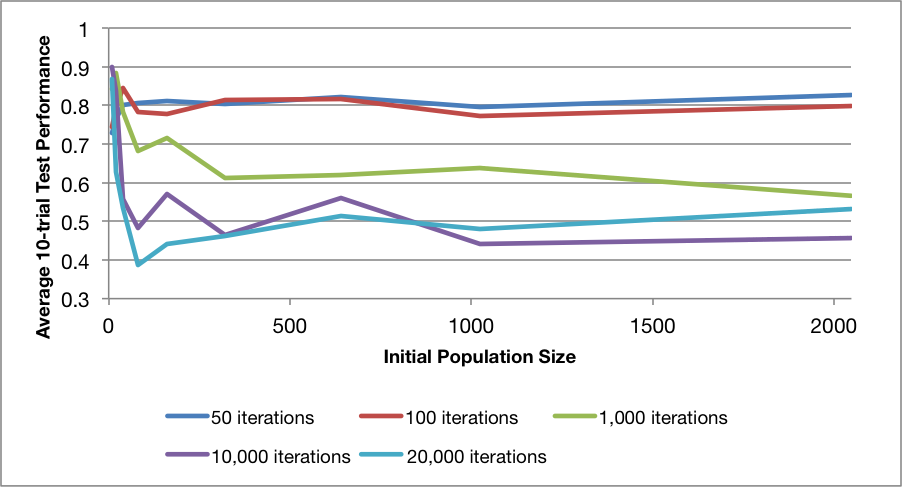
\includegraphics[width=\textwidth]{pics/popsize}
    \caption{Initial Population Size versus Average 10-trial Test Performance for Various Iteration Counts}
    \label{fig:popsize}
\end{figure}

I expected larger populations to have better performance for GA compared to smaller populations as a larger sample should capture a more representative snapshot of the population. 

Experiment results (displayed in Figure \ref{fig:popsize}), however, appears to show that beyond some initial variation, performance is more-or-less constant as initial population size increases. This makes sense as the network is limited in terms of size of distinct parameters so adding more members to the initial population does not contribute significant new information or diversity.

It is interesting to see that there is overfitting with GA as an increased number of iterations results in improved train accuracy yet decreased test performance. It appears choosing a smaller initial population size may be a method to combat parameters overfitting slightly.



\subsubsection{Neural network train runtime}

\begin{figure}[h!]
    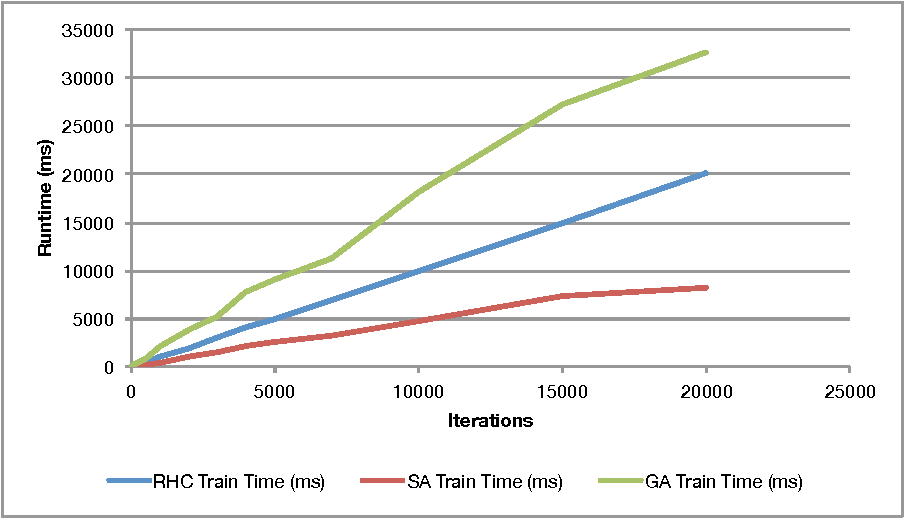
\includegraphics[width=\textwidth]{pics/runtime}
    \caption{Neural network runtime over 20,000 iterations for various optimization algorithms}
\end{figure}

There is a very clear linear relationship of runtime versus iterations.\footnote{$runtime \propto iterations$} Per-iteration runtime was lowest for SA and highest for GA. This aligns with what we may expect as GA is performing the most work (crossover and evaluation). Backpropogation is definitely still the fastest optimization technique but SA was very competitive.




\section{Phase 2: Optimization Problems}
\subsection{Problems chosen for optimization}

\subsubsection{Travelling salesman problem (GA)}
TSP is the problem of finding the optimal Hamiltonian cycle in a graph. This problem is NP-complete. Modern optimization techniques can approximate a solution within 2-3\% of the actual solution. As TSP is implemented in ABIGAIL, optimization is performed by computing the sum distance of a Hamiltonian cycle and then optimizing over the inverse. I suspect GA will perform well on this problem given the structures of the underlying problem where I can see how combining two short paths has a chance at producing a new instance that may have a shorter overall path.


\subsubsection{Count ones (SA)}
Count Ones is a very simple problem that attempts to count the number of 1's in a size n bitstring. I suspect that GA will not perform as well as SA on this problem as it does not have much structure. I suspect SA will perform well as there are many local minima (as one can flip single bits in the middle of a bitstring).

\subsubsection{Knapsack problem (MIMIC)}
The Knapsack problem\footnote{In order to run the experiment, the number of items was varied while other parameters were kept constant ($copies = 4$, $max\ weight = 50$, $max\ volume = 50$)} is where one wants to choose items that sum to a certain max weight limit while maximizing the value of those items. I suspect MIMIC will perform well on this problem as the Knapsack has structure in that the choice to add an item to the knapsack is conditionally dependent on the items in the bag currently. This structure can be approximated using dependency trees.

\subsection{Definitions and purposes of analysis}
What does better mean? We can define it in terms of runtime to achieve some threshold performance, we can define it to mean eventual performance, we can define it to mean correctness, etc. As each optimization problem highlights different performance characteristsics, this report will conduct this analysis by defining better to be \textbf{\textit{performance on a problem as a function over varying problem sizes}}. This definition was chosen in order to highlight how various optimization problems perform as problems grow larger, which should hopefully highlight the differences between algorithm performance as problems grow more complex (as do real world problems).


\subsection{Results and analysis}

\subsubsection{Travelling salesman problem}

It is apparent when scores are normalized that GA is very well suited to TSP. This follows from the reasoning presented above where that TSP is easily digested into sub-problems and then combined (e.g. TSP solution for some partition of cities). GA combines smaller sub-paths through cities through various iterations in order to converge on an optimal path. I am surprised by the relatively poor performance of MIMIC compared to other algorithms. I suspect this is because the structure behind TSP is not easily modeled as a set of dependency trees. I also suspect that MIMIC and SA performed poorly given the large size of the optimization space ($n!$ paths for $n$ cities).

\begin{figure}[h!]
    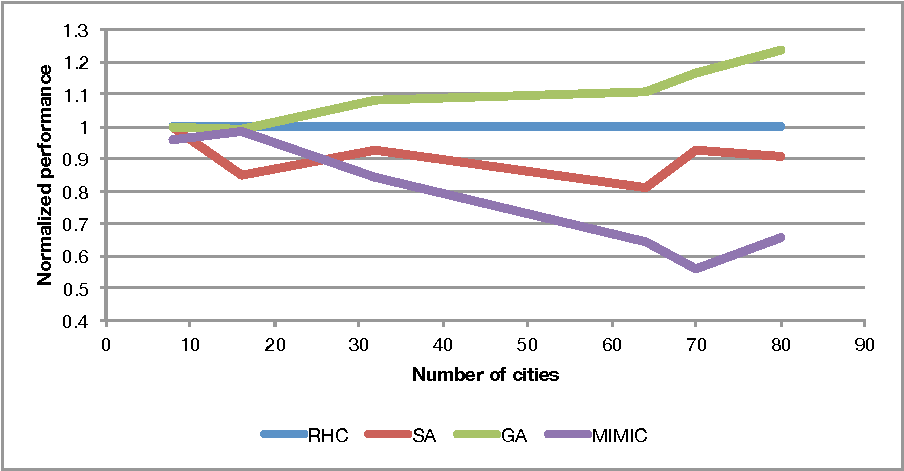
\includegraphics[width=\textwidth]{pics/tsp}
    \caption{TSP performance for various optimization algorithms, normalized to RHC performance baseline}
\end{figure}

\subsubsection{Count ones}

MIMIC performed well alongside RHC but SA was very close behind. Interestingly, GA performs poorly at this task. With no structure, it is not surprising that GA performs poorly while RHC and SA both perform well. Dependency structures aren't very helpful here, as mutating a bit shouldn't vary the result too greatly. However, the runtime for SA was orders of magnitude faster than MIMIC. This highlights strength of SA or RHC – when problems lack structure, SA and RHC can efficiently reach a near optimal solution rapidly. Note that here, SA had less runtime than RHC so given how close resulting performance is, it makes sense to use SA over more iterations.

\begin{figure}[h!]
    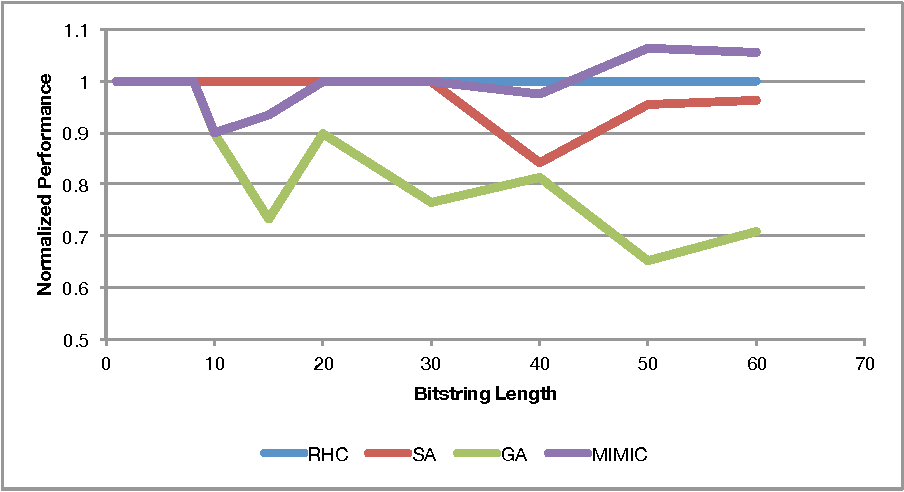
\includegraphics[width=\textwidth]{pics/countones}
    \caption{Count-ones performance over various optimization algorithms, normalized to RHC performance}
\end{figure}

\subsubsection{Knapsack problem}

Not surprisingly, MIMIC performs very well on the Knapsack problem. There is clear structure as described earlier that is captured well by dependency trees. It is interesting that GA did not perform anywhere close to the performance of MIMIC. This is perhaps because more structure is needed than the mutation/natural selection structure of GA problems. RHC and SA are very close in performance. This makes sense, as they both do not exploit structure, which appears to be key in order to solve the problem.

\begin{figure}[h!]
    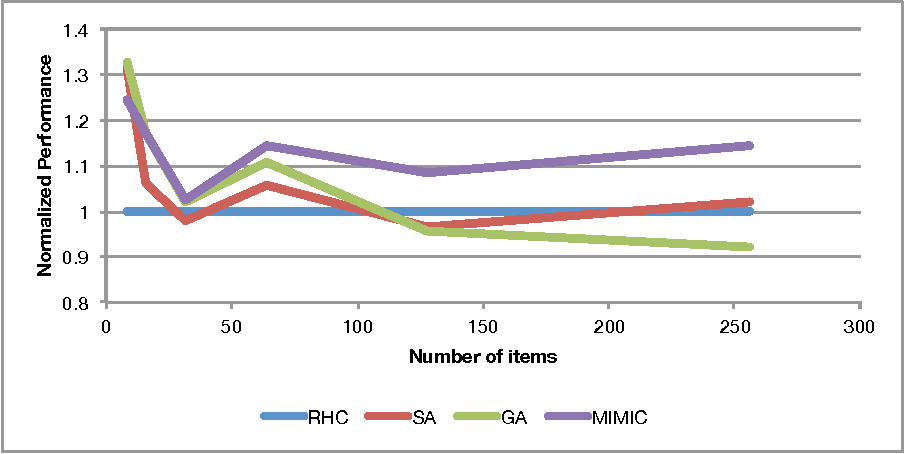
\includegraphics[width=\textwidth]{pics/knapsack}
    \caption{Knapsack problem performance over various optimization algorithms, normalized to RHC}
\end{figure}



\subsubsection{Optimization runtime}


\end{document}